\documentclass[11pt,a4paper]{article}
\usepackage[utf8]{inputenc}
\usepackage{graphicx}
\usepackage{hyperref}
\usepackage{listings}
\usepackage{xcolor}
\usepackage{geometry}
\usepackage{tikz}
\usepackage{amsmath}
\usepackage{enumitem}
\usepackage{multicol}
\usetikzlibrary{arrows,shapes,positioning}

\geometry{margin=0.85in}

\setlist{noitemsep, topsep=3pt}

\definecolor{codegreen}{rgb}{0,0.6,0}
\definecolor{codegray}{rgb}{0.5,0.5,0.5}
\definecolor{codepurple}{rgb}{0.58,0,0.82}
\definecolor{backcolour}{rgb}{0.95,0.95,0.92}

\lstdefinestyle{cstyle}{
    backgroundcolor=\color{backcolour},
    commentstyle=\color{codegreen},
    keywordstyle=\color{magenta},
    numberstyle=\tiny\color{codegray},
    stringstyle=\color{codepurple},
    basicstyle=\ttfamily\footnotesize,
    breakatwhitespace=false,
    breaklines=true,
    numbers=left,
    numbersep=5pt,
    showspaces=false,
    showstringspaces=false,
    showtabs=false,
    tabsize=2,
    aboveskip=4pt,
    belowskip=4pt
}

\title{\vspace{-1.5em}Spreadsheet Program \\ \large ACOP290 Lab Project\vspace{-0.5em}}
\author{
Vipulav Batra (24A1CSEB0024) \\
Sumant Varanasi (24A1CSEB0023)
}
\begin{document}

\maketitle
\vspace{-1em}

\section{Introduction}

A terminal-based spreadsheet program supporting a grid of up to 999 rows and 18,278 columns (A1--ZZZ999), with formula evaluation, automatic recalculation, and circular dependency detection.

\begin{multicols}{2}
\textbf{Core features:}
\begin{itemize}
    \item Integer cell values with ERR propagation
    \item Arithmetic operators: \texttt{+}, \texttt{-}, \texttt{*}, \texttt{/}
    \item Functions: SUM, MIN, MAX, AVG, STDEV, SLEEP
    \item 1D and 2D range support (e.g.\ \texttt{A1:B10})
    \item Dependency tracking \& auto-recalculation
    \item Circular dependency detection and rejection
    \item Scrollable 10$\times$10 viewport (scrolls by 10)
    \item Commands: \texttt{disable\_output}, \texttt{enable\_output}, \texttt{scroll\_to}
\end{itemize}
\end{multicols}

\section{Software Architecture}

\subsection{File Structure}

\begin{center}
\begin{tabular}{|l|p{8.5cm}|}
\hline
\textbf{File} & \textbf{Purpose} \\
\hline
\texttt{sheet.c/h}     & Core data structures (Cell, Sheet) and basic operations \\
\texttt{parser.c/h}    & Cell name parsing: A1 $\leftrightarrow$ (row, col); bijective base-26 columns \\
\texttt{formula.c/h}   & Expression evaluation and built-in function handling \\
\texttt{deps.c/h}      & Dependency graph, cycle detection, BFS recalculation \\
\texttt{main.c}        & User interface and command loop \\
\texttt{test\_suite.c} & Automated test suite (built via \texttt{make test}) \\
\texttt{Makefile}      & Targets: \texttt{all}, \texttt{test}, \texttt{run}, \texttt{report}\\
\hline
\end{tabular}
\end{center}

\subsection{System Architecture}

\begin{center}
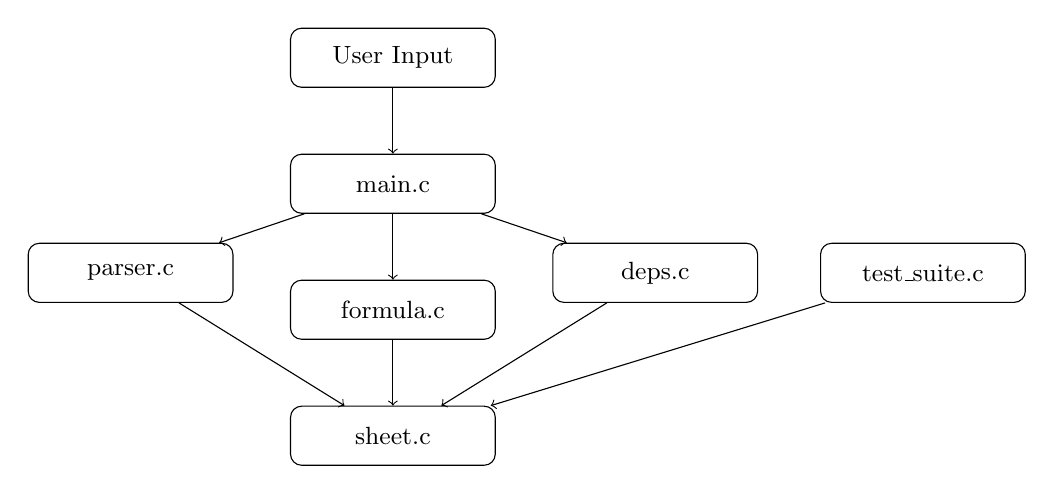
\begin{tikzpicture}[
    node distance=1.6cm,
    box/.style={rectangle, draw, rounded corners, minimum width=2.6cm, minimum height=0.75cm, font=\small}
]
\node[box] (user)    {User Input};
\node[box, below of=user]                        (main)    {main.c};
\node[box, below left of=main,  xshift=-2.2cm]   (parser)  {parser.c};
\node[box, below of=main]                        (formula) {formula.c};
\node[box, below right of=main, xshift=2.2cm]    (deps)    {deps.c};
\node[box, below of=formula]                     (sheet)   {sheet.c};
\node[box, right of=deps,       xshift=1.8cm]    (test)    {test\_suite.c};

\draw[->] (user)    -- (main);
\draw[->] (main)    -- (parser);
\draw[->] (main)    -- (formula);
\draw[->] (main)    -- (deps);
\draw[->] (parser)  -- (sheet);
\draw[->] (formula) -- (sheet);
\draw[->] (deps)    -- (sheet);
\draw[->] (test)    -- (sheet);
\end{tikzpicture}
\end{center}

\section{Key Data Structures}

\subsection{Cell}

The constant \texttt{CELL\_ERR\_VALUE} (\texttt{INT\_MIN}) serves as the error sentinel. Forward dependencies are capped at \texttt{MAX\_DEPS} (4096); reverse dependencies grow dynamically.

\begin{lstlisting}[style=cstyle, caption={Cell structure (sheet.h)}]
#define MAX_DEPS       4096
#define CELL_ERR_VALUE (-2147483647-1)  /* INT_MIN -- ERR sentinel */

typedef struct {
    int   value;       /* Current integer value                   */
    int   has_error;   /* Non-zero if cell is in ERR state        */
    char *formula;     /* Stored formula string (NULL if literal) */
    int  *deps;        /* Encoded cells this cell depends on      */
    int   dep_count;
    int  *rdeps;       /* Encoded cells that depend on this cell  */
    int   rdep_count;
    int   rdep_cap;    /* Allocated capacity of rdeps array       */
} Cell;
\end{lstlisting}

\subsection{Sheet}

\begin{lstlisting}[style=cstyle, caption={Sheet structure (sheet.h)}]
#define MAX_ROWS 999    #define MAX_COLS 18278
#define VIEW_ROWS 10    #define VIEW_COLS 10

typedef struct {
    int    rows, cols;         /* Sheet dimensions                 */
    Cell **cells;              /* 2-D array of Cell pointers       */
    int    view_row, view_col; /* Top-left corner of viewport      */
    int    output_enabled;     /* Flag for disable_output feature  */
} Sheet;
\end{lstlisting}

Cell positions are packed into a single integer: \texttt{encode(r,c) = r * MAX\_COLS + c}.

\section{Key Algorithms}

\subsection{Cycle Detection - DFS}

Before committing a new formula, a DFS checks whether any new dependency can reach the target cell. If so, the formula is rejected and the sheet is left unchanged.

\begin{lstlisting}[style=cstyle, caption={Cycle detection (deps.c)}]
static int creates_cycle(Sheet *s, int target, int *deps, int dep_count) {
    for (int i = 0; i < dep_count; i++)
        if (has_path(s, deps[i], target, visited))
            return 1;
    return 0;
}
\end{lstlisting}

\subsection{Recalculation - BFS over Reverse Dependencies}

After any cell changes, all transitively-dependent cells are updated via BFS over the \texttt{rdeps} graph, limiting work to the affected subgraph: $O(V + E)$ per update instead of $O(N)$.

\begin{lstlisting}[style=cstyle, caption={BFS recalculation (deps.c)}]
static void recalc_downstream(Sheet *sheet, int start_enc) {
    /* BFS queue seeded with start_enc.
       Each dequeued cell is re-evaluated; its rdeps are enqueued. */
}
\end{lstlisting}

\subsection{Column Naming - Bijective Base-26}

Standard base-26 has no zero digit, so column indices use bijective base-26: A=1, \ldots, Z=26, AA=27, \ldots, ZZZ=18278, giving unique Excel-compatible labels.

\section{User Interface}

The viewport shows 10$\times$10 cells and scrolls by 10 per keystroke. Every command prints its execution time. Launch with \texttt{./sheet \textit{rows} \textit{cols}}.

\begin{center}
\begin{tabular}{|l|l|}
\hline
\textbf{Input} & \textbf{Action} \\
\hline
\texttt{w / s / a / d}   & Scroll up / down / left / right by 10 \\
\texttt{scroll\_to A1}   & Jump viewport to a specific cell \\
\texttt{disable\_output} & Suppress display (useful for batch input) \\
\texttt{enable\_output}  & Re-enable display \\
\hline
\end{tabular}
\end{center}

\section{Test Suite}

\texttt{test\_suite.c} is compiled and run via \texttt{make test}. It covers arithmetic, division-by-zero, circular dependencies, function evaluation, ERR cascading, and range validation.

\begin{verbatim}
The format is:
Test: Addition 
Input:
A1=2
B1 = A1+1
Expected : 3
Output: Spreadsheets showing th steps
\end{verbatim}

\subsection*{Note}
If the user wants to compile again or just access the source files \\
Just type 'make clean' in the terminal

\section{Edge Cases, Error Handling, and Challenges}

\subsection{Edge Cases Covered by Test Suite}

The test suite is designed to validate correctness under both normal and extreme conditions. Key edge cases include:

\begin{itemize}
    \item \textbf{Division by Zero:} Expressions such as \texttt{A1 = 1/0} correctly produce \texttt{ERR}, ensuring safe arithmetic evaluation.
    
    \item \textbf{Invalid Cell References:} Inputs like \texttt{X9999=5} or \texttt{A0=5} are rejected as out-of-bounds, preventing undefined behavior.
    
    \item \textbf{Invalid Commands:} Non-recognized inputs (e.g.\ \texttt{hello}) are handled gracefully with error messages.
    
    \item \textbf{Reverse and Invalid Ranges:} Cases such as \texttt{MAX(A5:A1)} are detected and flagged as invalid ranges.
    
    \item \textbf{Circular Dependencies:} Both direct (\texttt{A1=A1+1}) and indirect cycles are detected using DFS and rejected before execution.
    
    \item \textbf{Error Propagation:} When a cell enters an \texttt{ERR} state, all dependent cells automatically reflect the error.
    
    \item \textbf{Recalculation Chains:} Multi-level dependencies (e.g.\ \texttt{A1 $\rightarrow$ B1 $\rightarrow$ C1}) are updated correctly when a base value changes.
    
    \item \textbf{Selective Recalculation:} The system avoids unnecessary recomputation when dependencies are removed or overridden.
    
    \item \textbf{Function Evaluation:} Aggregate functions such as \texttt{SUM}, \texttt{AVG}, \texttt{MIN}, and \texttt{MAX} are validated for both 1D and 2D ranges.
    
    \item \textbf{Sleep Function Handling:} \texttt{SLEEP(n)} ensures delayed execution without breaking dependency tracking.
    
    \item \textbf{UI Commands:} Commands like \texttt{disable\_output}, \texttt{enable\_output}, and scrolling operations are tested for correctness.
\end{itemize}

\subsection{Error Handling Strategy}

The spreadsheet uses a consistent error-handling model:

\begin{itemize}
    \item All errors are represented internally using a sentinel value (\texttt{INT\_MIN}).
    \item A separate \texttt{has\_error} flag ensures clarity between valid values and error states.
    \item Errors propagate through dependencies automatically during BFS recalculation.
    \item Invalid operations do not modify the sheet state, preserving consistency.
\end{itemize}

\subsection{Challenges Faced}

During development, several non-trivial challenges were encountered:

\begin{itemize}
    \item \textbf{Cycle Detection Efficiency:} Ensuring accurate cycle detection without significant performance overhead required careful DFS design.
    
    \item \textbf{Dependency Management:} Maintaining both forward (\texttt{deps}) and reverse (\texttt{rdeps}) graphs while avoiding memory issues was complex.
    
    \item \textbf{Efficient Recalculation:} Designing BFS-based updates to limit recomputation only to affected cells required precise graph traversal logic.
    
    \item \textbf{Parsing Expressions:} Handling formulas with mixed operators, functions, and ranges while maintaining correctness was challenging.
    
    \item \textbf{Range Handling:} Supporting both 1D and 2D ranges (e.g.\ \texttt{A1:B10}) introduced edge cases in validation and iteration.
    
    \item \textbf{Error Propagation:} Ensuring consistent propagation across multiple dependency levels without redundant computation required careful design.
    
    \item \textbf{Terminal UI Constraints:} Implementing a scrollable viewport within terminal limitations while keeping output readable required thoughtful formatting.
    
    \item \textbf{Testing Complexity:} Capturing and validating program output via \texttt{popen()} required handling formatting variations and ensuring robust string matching.
\end{itemize}

\section{Conclusion}

The program implements a full dependency graph with DFS cycle detection, BFS recalculation, ERR propagation, and bijective base-26 column naming. The modular six-file architecture keeps each concern isolated and easy to extend.

\section{Resources}
\begin{itemize}
    \item GitHub: \url{https://github.com/Vipulav-me/ACOP290-Project}
\end{itemize}

\end{document}
